
\subsection{mSMCR-based optimization strategies}\label{S:mSMCR}

This section presents portfolio optimization strategies based on the
mSMCR dispersion measure, \ie,
\begin{equation}
    \mSMCR = \sum_{l=1}^L \cK_l \times \SMCR_{\alpha_l},
    \label{smcr0}
\end{equation}
where $\{\cK_l\}_{l=1,\cdots,L}$ is a set of positive coefficients normalized to unit (the mixture coefficients),
$\{\alpha_l\}_{l=1,\cdots,L}$ is a set of distinct confidence levels  and
\begin{equation}
    \SMCR_\alpha(r) = \min_u\left( u + \frac{1}{1-\alpha} \left\| (-\br -u)^+ \right\|_2 \right),
    \label{smcrS}
\end{equation}
where $\br = r - \mE[r]$ is the detrended rate of return and $\|\cdot\|_2 = (\mE[|\cdot|^2])^{1/2}$ is the $L^2$-norm.

\BackToContents


\subsubsection{mSMCR dispersion measure}

This subsection presents the SOCP approximation for \mSMCR\ dispersion measure.

Given a set $\{r_i\}_{i=1,\cdots,N}$ of observed rates of return, Eq.~(\ref{smcrS}) can be rewritten as
\begin{equation}
    \SMCR_\alpha = \min_u\left[ u + \frac{1}{(1-\alpha)\sqrt{N}}\left( \sum_{i=1}^N \left[(-u - \br_i)^+\right]^2 \right)^{1/2} \right].
    \label{smcr1:1}
\end{equation}
It is straightforward to show that, Eq.~(\ref{smcr1:1}) can be transformed into the following SOCP problem,

\bigskip
\noindent Minimize over $\{u, \eta, \{s_i\}_{i=1,\cdots,N}\}$
\begin{subequations}\label{smcr1}
\begin{align}
    &g = u + \frac{\eta}{1-\alpha} , \label{smcr1a} \\
    \st &\left( \frac{1}{N}\sum_{i=1}^N s_i^2 \right)^{1/2} \leq \eta, \label{smcr1b} \\
        &s_i + u \geq -\br_i, \label{smcr1c} \\
        &s_i \geq 0, \label{smcr1d} \\
        &\eta \geq 0, \label{smcr1e} \\
        &u \geq 0, \label{smcr1f}
\end{align}
\end{subequations}

\noindent where $\br_i$ is the i-th detrended rate of return, \ie\ $\br_i = r_i - \frac{1}{N}\sum_{j=1}^N r_j$.
Then, we have
\begin{subequations}\label{smcr2}
\begin{align}
    \SMCR_\alpha &= g^*, \label{smcr2a} \\
    \SMVaR_\alpha & = u^*, \label{smcr2b}
\end{align}
\end{subequations}

\noindent where $^*$ denotes the solutions of SOCP problem.

Further, \mSMCR\ is given by the sum from Eq.~(\ref{smcr0}).
In total there are $L$ decoupled SOCP problems, one for each mixture element.

Note that, the transformation of Eq.~(\ref{smcr1:1}) into the SOCP problem from Eqs.~(\ref{smcr1})
is at the core of all \mSMCR-based optimal portfolio algorithms. However, in these cases all the mixture elements
will be coupled in a single SOCP problem.

\BackToContents

\subsubsection{mSMCR optimal portfolio}
The optimization is described by Eqs.~(\ref{gg1}) from Sec.~\ref{strategies} point~\ref{OptRisk},
where $\rho$ is given by \mSMCR\ from Eq.~(\ref{smcr0}).
It is the following SOCP problem.

\bigskip
\noindent Minimize over $\{ \{w_k\}_{k=1,\cdots,M}, \{ u_l, \eta_l, \{s_{li}\}_{i=1,\cdots,N} \}_{l=1,\cdots,L}\}$
\begin{subequations}\label{smcr3}
\begin{align}
    &g = \sum_{l=1}^L \cK_l \left( u_l + \frac{\eta_l}{1 - \alpha_l}  \right), \label{smcr3a} \\
    \st &\left( \frac{1}{N}  \sum_{i=1}^N s_{li}^2 \right)^{1/2} \leq \eta_l, \label{smcr3b} \\
        &s_{li} + u_l + \sum_{k=1}^M w_k \br_{ki} \geq 0, \label{smcr3c} \\
        &\sum_{k=1}^M w_k \mu_k \geq \mu, \label{smcr3d} \\
        &\sum_{k=1}^M w_k = 1, \label{smcr3e} \\
        &s_{li} \geq 0, \label{smcr3f} \\
        &\eta_l \geq 0, \label{smcr3h} \\
        &u_l \geq 0, \label{smcr3i} \\
        &w_k \geq 0, \label{smcr3g}
\end{align}
\end{subequations}

\noindent where $\mu$ in Eq.~(\ref{smcr3d}) is the portfolio targeted expected rate of return, $\mu_k$ for $k=1,\cdots,M$
are the portfolio components expected rate of returns and $\br_{ki}$ in Eq.~(\ref{smcr3c}) is the $i$-th detrended observation of the
$k$-th portfolio component rate of return.
Then, we have
\begin{subequations}\label{smcr4}
\begin{align}
    \RR &= \sum_{k=1}^M w_k^* \mu_k, \label{smcr4a} \\
    \mSMCR &= g^*, \label{smcr4b} \\
    \SMCR_{\alpha_l} &= u_l^* + \frac{\eta_l^*}{1-\alpha_l} , \label{smcr4c} \\
    \SMVaR_{\alpha_l} &= u_l^*, \label{smcr4d}
\end{align}
\end{subequations}

\noindent where $^*$ denotes the solution of SOCP problem.
In addition to the optimal portfolio weights $\{w_k^*\}_{k=1,\cdots,M}$ and the expected rate of return $\RR$,
the SOCP solution provides information about the portfolio \mSMCR\ and its \SMCR\  and
associated \SMVaR\ components.

\bigskip
\noindent Here is an example, using the \azapy\ package, of how to compute the \mSMCR\ optimal portfolio.
The \mSMCR\ time horizon was set to one quarter and the calibration is performed using the prior 3.25 years of
close-adjusted historical prices (default settings).
For more details see the package documentation at \azapydoc.

\lstinputlisting[language=Python]{../PyScripts/SMCR_RiskOptim.py}

\BackToContents

\subsubsection{Minimum mSMCR portfolio}
Following the results from Sec.~\ref{strategies} point~\ref{MinRisk},
the algorithm to compute the optimal portfolio with minimum \mSMCR\ is given by the SOCP problem from Eqs.~(\ref{smcr3}) where
$\mu$ from r.h.s. of Eq.~(\ref{smcr3d}) is set to a value equal to the smallest expected rate of
return among the portfolio components, \ie\ $\mu = \min_k\{\mu_k\}$.

\bigskip
\noindent Here is an example, using the \azapy\ package, of how to compute the minimum \mSMCR\ portfolio.
The \mSMCR\ time horizon was set to one quarter and the calibration is performed using the prior 3.25 years of
close-adjusted historical prices (default settings).
For more details see the package documentation at \azapydoc.

\lstinputlisting[language=Python]{../PyScripts/SMCR_MinRisk.py}

\BackToContents

\subsubsection{mSMCR optimal portfolio for targeted risk value}
The optimization is described by Eqs.~(\ref{gg2}) from Sec.~\ref{strategies} point~\ref{TargetRisk}, where
$\rho$ is given by \mSMCR\ from Eq.~(\ref{smcr0}).
It is the following SOCP problem.

\bigskip
\noindent Maximize over $\{ \{w_k\}_{k=1,\cdots,M}, \{ u_l, \eta_l, \{ s_{li}\}_{i=1,\cdots,N} \}_{l=1,\cdots, L}\}$
\begin{subequations}\label{smcr5}
\begin{align}
    &g = \sum_{k=1}^M w_k \mu_k, \label{smcr5a} \\
    \st &\left( \frac{1}{N} \sum_{i=1}^N s_{li}^2 \right)^{1/2} \leq \eta_l, \label{smcr5b} \\
        &s_{li} + u_l + \sum_{k=1}^M w_k \br_{ki} \geq 0, \label{smcr5c} \\
        &\sum_{l=1}^L \cK_l\left( u_l + \frac{\eta_l}{1 - \alpha_l} \right) = \mSMCR_0, \label{smcr5d} \\
        &\sum_{k=1}^M w_k = 1, \label{smcr5e} \\
        &s_{li} \geq 0, \label{smcr5f} \\
        &\eta_l \geq 0, \label{smcr5h} \\
        &u_l \geq 0, \label{smcr5i} \\
        &w_k \geq 0, \label{smcr5g}
\end{align}
\end{subequations}

\noindent where $\mSMCR_0$ in Eq.~(\ref{smcr5d}) is the portfolio targeted \mSMCR\ dispersion value.
Then, we have
\begin{subequations}\label{smcr6}
\begin{align}
    \RR &= g^*, \label{smcr6a} \\
    \SMCR_{\alpha_l} &= u_l^* + \frac{\eta_l^*}{1-\alpha_l} , \label{smcr6b} \\
    \SMVaR_{\alpha_l} &= u_l^*, \label{smcr6c}
\end{align}
\end{subequations}

\noindent where $^*$ denotes the solution of SOCP problem.
In addition to the optimal portfolio weights $\{w_k^*\}_{k=1,\cdots,M}$ and the portfolio expected rate of return $\RR$,
the SOCP solution provides information about the value of the \SMCR\ and associated \SMVaR\
components of $\mSMCR_0$, although, this information is likely to be known at the outset.

\bigskip
\noindent Here is an example, using the \azapy\ package, of how to compute the optimal portfolio
with the same \mSMCR\ as the equal weighted portfolio.
The \mSMCR\ time horizon was set to one quarter and the calibration is performed using the prior 3.25 years of
close-adjusted historical prices (default settings).
For more details see the package documentation at \azapydoc.

\lstinputlisting[language=Python]{../PyScripts/SMCR_InvNrisk.py}

\BackToContents

\subsubsection{mSMCR optimal portfolio for fixed risk-aversion factor}
The optimization is described by Eqs.~(\ref{gg3}) from Sec.~\ref{strategies} point~\ref{RiskAverse},
where $\rho$ is given by \mSMCR\ from Eq.~(\ref{smcr0}).
It is the following SOCP problem.

\bigskip
\noindent Maximize over $\{ \{w_k\}_{k=1,\cdots,M}, \{ u_l, \eta_l, \{s_{li}\}_{i=1,\cdots,N} \}_{l=1,\cdots,L}\}$
\begin{subequations}\label{smcr7}
\begin{align}
    &g = \sum_{k=1}^M w_k\mu_k - \lambda \sum_{l=1}^L \cK_l \left( u_l + \frac{\eta_l}{1 - \alpha_l}  \right), \label{smcr7a} \\
    \st &\left( \frac{1}{N} \sum_{i=1}^N s_{li}^2 \right)^{1/2} \leq \eta_l, \label{smcr7b} \\
        &s_{li} + u_l + \sum_{k=1}^M w_k \br_{ki} \geq 0, \label{smcr7c} \\\
        &\sum_{k=1}^M w_k = 1, \label{smcr7d} \\
        &s_{li} \geq 0, \label{smcr7e} \\
        &\eta_l \geq 0, \label{smcr7g} \\
        &u_l \geq 0, \label{smcr7h} \\
        &w_k \geq 0, \label{smcr7f}
\end{align}
\end{subequations}

\noindent where $\lambda$ from Eqs.~(\ref{smcr7a}) is the risk-aversion factor.
Then, we have
\begin{subequations}\label{smcr8}
\begin{align}
    \RR &= \sum_{k=1}^M w_k^* \mu_k, \label{smcr8a} \\
    \mSMCR &= \frac{\RR - g^*}{\lambda}, \label{smcr8b} \\
    \SMCR_{\alpha_l} &= u_l^* + \frac{\eta_l^*}{1-\alpha_l} , \label{smcr8c} \\
    \SMVaR_{\alpha_l} &= u_l^*, \label{smcr8d}
\end{align}
\end{subequations}

\noindent where $^*$ denotes the solution of SOCP problem.
In addition to the portfolio weights $\{w_k^*\}_{k=1,\cdots,M}$ and the portfolio expected rate of return $\RR$,
the SOCP solution provides information about portfolio $\mSMCR$ and its \SMCR\  and
associated \SMVaR\ components.

\bigskip
\noindent Here is an example, using the \azapy\ package, of how to compute the optimal portfolio
for a given value of the risk-aversion factor $\lambda$.
The \mSMCR\ time horizon was set to one quarter and the calibration is performed using the prior 3.25 years of
close-adjusted historical prices (default settings).
For more details see the package documentation at \azapydoc.

\lstinputlisting[language=Python]{../PyScripts/SMCR_Averse.py}

\BackToContents

\subsubsection{mSMCR-Sharpe optimal portfolio - maximization solution}
This optimization targets the maximization of \mSMCR-Sharpe ratio.
It is described by Eqs.~(\ref{gg4}) from Sec.~\ref{strategies} point~\ref{MaxSharpe},
where $\rho$ is given by \mSMCR\ from Eq.~(\ref{smcr0}).
The optimization can be formulated as an SOCP problem
if Eq.~(\ref{gg6b}) can be transformed to a second order cone constraint. This can be achieved by introducing the
variable transformations $\bw_k = t w_k$, $\bs_{li} = t s_{li}$, $\bbeta_l = t \eta_l$  and $\bu_l = t u_l$.
Then, the SOCP problem can be written as follows.

\bigskip
\noindent Maximize over $\{ \{\bw_k\}_{k=1,\cdots,M}, \{ \bu_l, \bbeta_l, \{\bs_{li}\}_{i=1,\cdots,N} \}_{l=1,\cdots,L}, t\}$
\begin{subequations}\label{smcr9}
\begin{align}
    &g = \sum_{k=1}^M \bw_k \mu_k - \mu_0 t, \label{smcr9a} \\
    \st &\left( \frac{1}{N} \sum_{i=1}^N \bs_{li}^2 \right)^{1/2} \leq \bbeta_l, \label{smcr9b} \\
        &\bs_{li} + \bu_l + \sum_{k=1}^M \bw_k \br_{ki} \geq 0, \label{smcr9c} \\
        &\sum_{l=1}^L \cK_l \left( \bu_l + \frac{\bbeta_l}{1 - \alpha_l}  \right) = 1, \label{smcr9d} \\
        &\sum_{k=1}^M \bw_k - t = 0, \label{smcr9e} \\
        &t \geq 0, \label{smcr9i} \\
        &\bs_{li} \geq 0, \label{smcr9f} \\
        &\bu_l \geq 0, \label{smcr9j} \\
        &\bbeta_l \geq 0, \label{smcr9h} \\
        &\bw_k \geq 0, \label{smcr9g}
\end{align}
\end{subequations}

\noindent where $\mu_0$ from Eq.~(\ref{cvar11a}) is the risk-free rate accessible to the investor.
Then, we have
\begin{subequations}\label{smcr10}
\begin{align}
    w_k &= \frac{\bw_k^*}{t^*}, \label{smcr10a} \\
    \RR &= \frac{g^*}{t^*}  + \mu_0, \label{smcr10c} \\
    \Sharpe &= g^*, \label{smcr10b} \\
    \mSMCR &= \frac{1}{t^*}, \label{smcr10d} \\
    \SMCR_{\alpha_l} &= \frac{1}{t^*}\left( \bu_l^* + \frac{\bbeta_l^*}{1-\alpha_l}  \right), \label{smcr10e} \\
    \SMVaR_{\alpha_l} &= \frac{\bu_l^*}{t^*} , \label{smcr10f}
\end{align}
\end{subequations}

\noindent where $^*$ denotes the solution of SOCP problem.
In addition to the optimal portfolio weights $\{w_k\}_{k=1,\cdots,M}$, expected rate of return $\RR$ and \mSMCR-Sharpe ratio $\Sharpe$,
the SOCP solution provides information about the portfolio \mSMCR\ and its \SMCR\  and associated \SMVaR\ components.

\bigskip
\noindent Here is an example, using the \azapy\ package, of how to compute the \mSMCR-Sharpe optimal portfolio using the maximization
of \mSMCR-Sharpe ratio.
The \mSMCR\ time horizon was set to one quarter and the calibration is performed using the prior 3.25 years of
close-adjusted historical prices (default settings).
For more details see the package documentation at \azapydoc.

\lstinputlisting[language=Python]{../PyScripts/SMCR_Sharpe.py}

\BackToContents

\subsubsection{mSMCR-Sharpe optimal portfolio - minimization solution}
This optimization targets the minimization of the inverse of \mSMCR-Sharpe ratio.
It is described by Eqs.~(\ref{gg8}) from Sec.~\ref{strategies} point~\ref{MinSharpe}, where
$\rho$ is given by \mSMCR\ from Eq.~(\ref{smcr0}).
The optimization can be formulated as an SOCP problem if Eq.~(\ref{gg8a}) can be expressed as a second order cone constraint. This can be achieved by
introducing the variable transformations
$\bw_k = t w_k$, $\bs_{li} = t s_{li}$, $\bbeta_l = t \eta_l$ and $\bu_l = t u_l$.
Then, the SOCP problem can be written as follows.

\bigskip
\noindent Minimize over $\{ \{\bw_k\}_{k=1,\cdots,M}, \{ \bu_l, \bbeta_l, \{\bs_{li}\}_{i=1,\cdots,N} \}_{l=1,\cdots,L}, t\}$
\begin{subequations}\label{smcr11}
\begin{align}
    &g = \sum_{l=1}^L \cK_l \left( \bu_l + \frac{\bbeta_l}{1 - \alpha_l}  \right), \label{smcr11a} \\
    \st &\left( \frac{1}{N} \sum_{i=1}^N \bs_{li}^2 \right)^{1/2} \leq \bbeta_l, \label{smcr11b} \\
        &\bs_{li} + \bu_l + \sum_{k=1}^M \bw_k \br_{ki} \geq 0, \label{smcr11c} \\
        &\sum_{k=1}^M \bw_k \mu_k - \mu_0 t = 1, \label{smcr11d} \\
        &\sum_{k=1}^M \bw_k - t = 0, \label{smcr11e} \\
        &t \geq 0, \label{smcr11j} \\
        &\bs_{li} \geq 0, \label{smcr11f} \\
        &\bu_l \geq 0, \label{smcr11i} \\
        &\bbeta_l \geq 0, \label{smcr11h} \\
        &\bw_k \geq 0, \label{smcr11g}
\end{align}
\end{subequations}

\noindent where $\mu_0$ from Eq.~(\ref{smcr11d}) is the risk-free rate accessible to the investor.
Then, we have
\begin{subequations}\label{smcr12}
\begin{align}
    w_k &= \frac{\bw_k^*}{t^*}, \label{smcr12a} \\
    \RR &= \frac{1}{t^*} + \mu_0, \label{smcr12c} \\
    \Sharpe &= \frac{1}{g^*}, \label{smcr12b} \\
    \mSMCR &= \frac{g^*}{t^*} , \label{smcr12d} \\
    \SMCR_{\alpha_l} &= \frac{1}{t^*}\left( \bu_l^* + \frac{\bbeta_l^*}{1-\alpha_l}  \right), \label{smcr12e} \\
    \SMVaR_{\alpha_l} &= \frac{\bu_l^*}{t^*} , \label{smcr12f}
\end{align}
\end{subequations}

\noindent where $^*$ denotes the solution of SOCP problem.
In addition to the optimal portfolio weights $\{w_k\}_{k=1,\cdots,M}$, expected rate of return $\RR$ and \mSMCR-Sharpe ratio $\Sharpe$,
the SOCP solution provides information about the portfolio \mSMCR\ and its \SMCR\ components and associated \SMVaR\ values.

\bigskip
\noindent Here is an example, using the \azapy\ package, of how to compute the \mSMCR-Sharpe optimal portfolio using the minimization
of the inverse of \mSMCR-Sharpe ratio.
The \mSMCR\ time horizon was set to one quarter and the calibration is performed using the prior 3.25 years of
close-adjusted historical prices (default settings).
For more details see the package documentation at \azapydoc.

\lstinputlisting[language=Python]{../PyScripts/SMCR_InvSharpe.py}

\BackToContents

\subsubsection{mSMCR frontiers}

Here is an example of how to compute the \mSMCR\ frontiers using the \azapy\
package. The \mSMCR\ time horizon was set to one quarter and the calibration is performed using the prior 3.25 years of
close-adjusted historical prices (default settings).
For more details see the package documentation at \azapydoc.

The script produces the plots in Figs. \ref{SMCR_fig1a} and \ref{SMCR_fig1b}
for historical data collected up to 2021-07-27.

\lstinputlisting[language=Python]{../PyScripts/SMCR_frontiers.py}

\begin{figure}[H]
\centering
\begin{subfigure}{.5\textwidth}
  \centering
  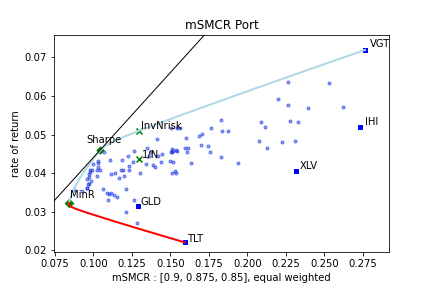
\includegraphics[width=.95\linewidth]{../figs/mSMCRFrontier1.png}
  \caption{Rate of return vs. \mSMCR}
  \label{SMCR_fig1a}
\end{subfigure}%
\begin{subfigure}{.5\textwidth}
  \centering
  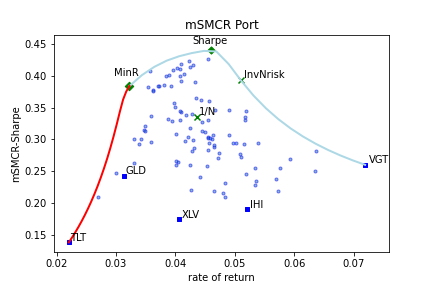
\includegraphics[width=.95\linewidth]{../figs/mSMCRFrontier2.png}
  \caption{\mSMCR-Sharpe vs. rate of return}
  \label{SMCR_fig1b}
\end{subfigure}
\caption{\mSMCR\ : [$\alpha=(0.9, 0.875, 0.85)$, equal weighted] frontiers.}
\label{SMCR_fig1}
\end{figure}

\BackToContents

\subsubsection{Backtesting mSMCR-Sharpe optimal portfolio}

Here is an example, using \azapy\ package, of computing a portfolio backtesting.
For this example, we have chosen a portfolio quarterly rebalanced according
to the maximization of \mSMCR-Sharpe ratio. At each rebalancing date,
the portfolio weights
are calibrated based on 3.25 years of prior historical market data (default settings).

Other rebalancing strategies can be considered
by changing the value of {\it rtype} parameter in the call of {\it set\_model} function below.
For more details see the package documentation at \azapydoc.

\lstinputlisting[language=Python]{../PyScripts/SMCR_Port.py}

\begin{figure}[H]
    \centering
    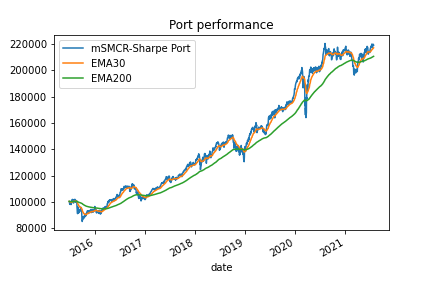
\includegraphics[width=.95\linewidth]{../figs/Port_mSMCR_Sharpe.png}
    \caption{Backtesting of quarterly rebalanced \mSMCR-Sharpe optimal portfolio,
    \mSMCR\ : [$\alpha=(0.975, 0.95, 0.9)$, equal weighted].}
    \label{SMCR_Port_fig}
\end{figure}

\BackToContents
